% -------------
\section{Template Certification}
\label{appendix:certification}

This section details the three checks of~\autoref{subsec:certification} (automated integrity
checks, an LLM screen, and expert certification) and their results.

\paragraph{Automated Integrity Checks.} We run every template at 500 seeds.
Every seed must generate an instance without error, regenerate it identically in a separate
process, keep the output format (numbered steps and one answer marker), print no malformed
expression, and pass the closure check: every printed calculation, recomputed from its printed
operands, gives its printed result at the printed precision.
We check by hand the lines that the closure check cannot parse (six line patterns in four
templates), and all 150 templates pass.

\paragraph{LLM Screen.} Three LLM judges from families outside the evaluated models,
\texttt{Grok 4.6}~\citep{grok46}, \texttt{MiniMax M3}~\citep{minimaxm3}, and
\texttt{MiMo-V2.5-Pro}, score each template's code and three of its instances with the prompt
below, at temperature 0, on physical plausibility, mathematical correctness, and pedagogical
clarity.
The screen gives each template one of three outcomes:
\begin{itemize}[nosep, leftmargin=*]
\item \textbf{Critical failure:} At least two judges flag the template for human review, or its
median score on any of the three is below 4.
\item \textbf{Controversial:} Not a critical failure, but the judges' scores on one of the three
have a population standard deviation above 0.5.
\item \textbf{Pass:} Neither of the above.
\end{itemize}

In the first pass, 126 templates pass, 13 are controversial, and 11 are critical failures, and the
judges agree on the review flag with Gwet's AC1 of 0.84~\citep{gwet2008}.
We check each claim in the judges' explanations against the code and the instances, and 34 of the
45 claims hold; after we revise the 24 flagged templates, 147 templates pass, 3 are controversial,
and none is a critical failure in the second pass (AC1 of 0.93).

Against the experts' first-round decisions, 15 of the 147 templates the screen passes are rejected
by a majority of their experts, so 10.2\% of the screen's passes are false positives.
On average, the median scores of experts and judges differ by 0.587 for physical plausibility,
0.187 for mathematical correctness, and 0.787 for pedagogical clarity, on the scale of 1 to 5.
The screen therefore guides revision, and the experts decide certification.

\begin{tcolorbox}[colback=gray!5, colframe=gray!40, boxrule=0.4pt, arc=2pt, left=5pt, right=5pt,
    top=5pt, bottom=5pt, breakable]
\ttfamily\small
You are an expert engineering professor and a senior Python developer acting as a peer reviewer for the EngTrace benchmark.\\
Your task is to meticulously evaluate a new problem template based on its source code and several example outputs.\\
Analyze the provided information and then respond ONLY with a single, valid JSON object that strictly adheres to the schema described in the user prompt. Do not add any explanatory text or markdown formatting around the JSON object.\\[3pt]
Please evaluate the following engineering problem template.\\[3pt]
\textbf{1. Template Source Code:}\\
python \{template\_code\}\\[3pt]
\textbf{2. Generated Instances from the Template:}\\
Instance 1: - Question: "\{q1\}" - Solution: "\{s1\}"\\
Instance 2: - Question: "\{q2\}" - Solution: "\{s2\}"\\
Instance 3: - Question: "\{q3\}" - Solution: "\{s3\}"\\[3pt]
\textbf{3. Evaluation Rubric \& JSON Schema:}\\
Evaluate the template based on the rubric below. The \texttt{human\_review\_flag} should be \texttt{true} if any score is less than 4. The \texttt{explanation} should be a concise, one-sentence justification for the scores and the flag.\\[3pt]
\{\\
\hspace*{1em}"physical\_plausibility\_score": \textless integer, a score from 1--5 based on whether the problem respects the laws of physics and engineering\textgreater,\\
\hspace*{1em}"mathematical\_correctness\_score": \textless integer, a score from 1--5 based on whether the equations and calculations are accurate\textgreater,\\
\hspace*{1em}"pedagogical\_clarity\_score": \textless integer, a score from 1--5 based on whether the problem statement is clear, unambiguous, and solvable\textgreater,\\
\hspace*{1em}"confidence\_score": \textless integer, a score from 1--5 indicating your confidence in this evaluation\textgreater,\\
\hspace*{1em}"human\_review\_flag": \textless boolean, true if the template requires human inspection, otherwise false\textgreater,\\
\hspace*{1em}"explanation": "\textless string, a concise, one-sentence justification for the scores and flag\textgreater"\\
\}
\end{tcolorbox}

\begin{table*}[t]
    \centering
    \small
    \renewcommand{\arraystretch}{1.1}
    \setlength{\tabcolsep}{4pt}
    \begin{tabular}{l p{0.205\textwidth} p{0.205\textwidth} p{0.205\textwidth} p{0.205\textwidth}}
        \toprule
        \rowcolor{gray!10}
        \textbf{Branch} & \textbf{Wrong Constant} & \textbf{Wrong Unit Conversion} &
        \textbf{Flipped Sign} & \textbf{Wrong Printed Result} \\
        \midrule
        Chemical & van der Waals pressure: $R$ with two digits transposed & annulus flow rate: kPa to Pa by a factor of 100 & heat of reaction: Hess's law reversed & first-order batch reactor: one printed time 4\% too high \\
        Electrical & Coulomb's law: $\varepsilon_0$ ten times too large & wave parameters: MHz to Hz by a factor of $10^5$ & C/D and D/C conversion: a delay written as an advance & mean and variance: one printed mean 0.2 too high \\
        Civil & Manning discharge: $R^{3/4}$ for $R^{2/3}$ & cantilever deflection: m to mm by a factor of 100 & effective stress: $\sigma' = \sigma + u$ & beam reactions: one printed reaction 4\% too high \\
        Industrial & safety stock: a two-sided $z$ for a one-sided one & M/M/1 time in system: hours to minutes by a factor of 100 & $\bar{x}$ and $R$ chart limits: the lower limit as center plus $A_2\bar{R}$ & process capability: one printed $C_p$ 6\% too high \\
        Mechanical & torsional shear stress: $J$ with $\pi/4$ for $\pi/2$ & hydrostatic pressure: kPa to Pa by a factor of 100 & U-tube manometer: the pipe-fluid column's sign flipped & natural frequency: one printed $\omega_n$ 4\% too high \\
        \bottomrule
    \end{tabular}
    \caption{\textbf{Planted defects.} The 20 planted defects, four per branch, each written into a
    real template of the branch; every expert of the branch reviews all four.}
    \label{tab:planted_defects}
\end{table*}

\paragraph{Expert Certification.} Three domain experts per branch each review the 30 templates of
their branch mixed with four planted defects.
Each expert sees the items in an order of their own, under opaque codes, and knows that planted
items exist but not which ones.
The experts do not see the screen's results, and they do not discuss a template before all three
have submitted.
Each planted defect is a real template of the branch with one error written into it
(\autoref{tab:planted_defects}); a wrong constant, unit conversion, or sign is carried through the
computation, the printed steps, and the answer, whereas a wrong printed result changes a single
printed line.
The planted defects test whether an expert catches a wrong number, through a constant, a unit
conversion, a sign, or a printed result; whether a question states everything its answer depends
on is examined separately, in the domain experts' reading of six near-miss templates
(\autoref{appendix:error_analysis}).

\paragraph{Certification App.} The experts work in a \texttt{Streamlit} web app
(\autoref{fig:certification_app}) built around the protocol:
\begin{itemize}[nosep, leftmargin=*]
\item \textbf{Blind hand check:} For each item, the expert solves one instance by hand; the app
shows the solution only once the expert enters an answer.
\item \textbf{Automatic comparison:} The app reports whether the answer is within 1\% of the gold
value and, on a mismatch, asks the expert to find which side is right.
\item \textbf{Multi-instance review:} Beside the gold solution, the expert can read the template's
source code and step through its other four instances, all generated in advance.
\item \textbf{Structured verdict:} The expert scores physical plausibility, mathematical
correctness, and pedagogical clarity from 1 to 5, approves or rejects, rates their confidence
from 1 to 5, and can name defect types from a fixed list: physics or scenario implausible;
governing equation or formula; constant or table value; unit or conversion; sign or direction; a
step that does not follow; final answer or unit wrong; question ambiguous or unsolvable; and
wording or formatting.
\item \textbf{Required justification:} The app accepts a rejection only with a note on what is
wrong and where and at least one defect type.
\end{itemize}

\begin{figure*}[tp]
    \centering
    \definecolor{framegray}{HTML}{EBDFD0}% the frame color of the overview figure
    \setlength{\fboxsep}{0pt}
    \setlength{\fboxrule}{0.5pt}
    {\small\textbf{(a)} Hand check}\par\smallskip
    \fcolorbox{framegray}{white}{%
        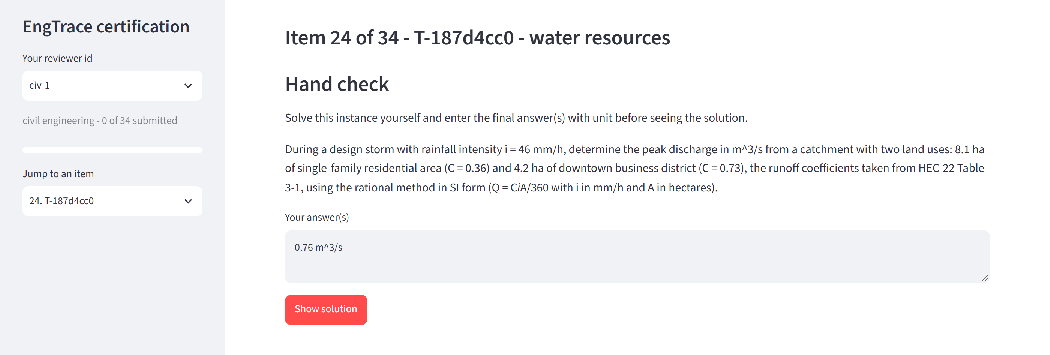
\includegraphics[width=0.985\textwidth]{figs/app_candidates/app-1-hand-check.pdf}}
    \par\bigskip
    {\small\textbf{(b)} Review}\par\smallskip
    \fcolorbox{framegray}{white}{%
        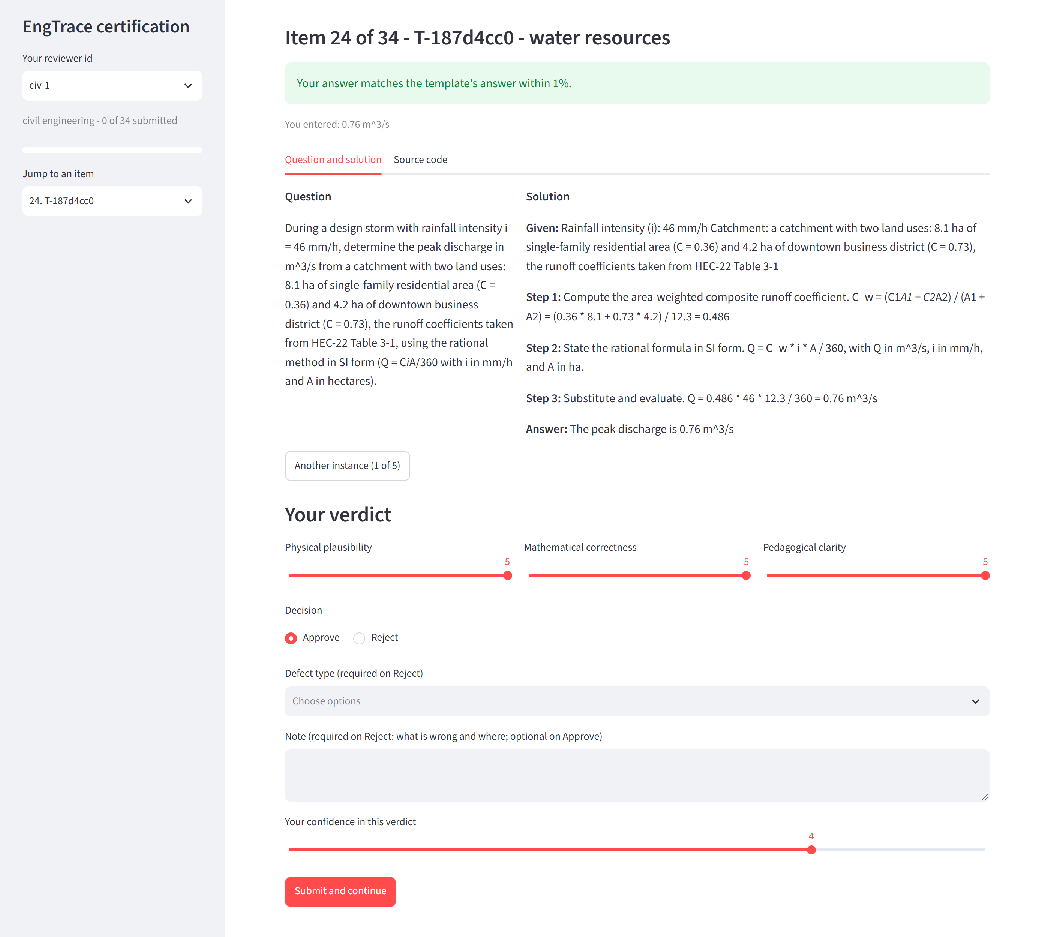
\includegraphics[width=0.985\textwidth]{figs/app_candidates/app-2-review.pdf}}
    \caption{\textbf{Certification app.}
    (a) The hand check: the expert enters the final answer with its unit before the solution is
    shown.
    (b) The review: the result of the hand check, the question beside the gold solution, the source
    code in a second tab, the template's other instances, and the verdict form.}
    \label{fig:certification_app}
\end{figure*}

\begin{table}[!htbp]
    \centering
    \small
    \setlength{\tabcolsep}{3.5pt}
    \begin{tabular}{l|ccc|ccc}
        \toprule
        \rowcolor{gray!10}
        \multirow{2}{*}{\textbf{Branch}} & \multicolumn{3}{c|}{\textbf{Approve or Reject}} &
        \multicolumn{3}{c}{\textbf{AC2 on Scores}} \\
        & $\kappa$ & \textbf{AC1} & \textbf{Agr.} &
        \textbf{Phys.} & \textbf{Math.} & \textbf{Ped.} \\
        \midrule
        Chemical & 0.492 & 0.776 & 77\% & 0.898 & 0.952 & 0.912 \\
        Electrical & 0.365 & 0.926 & 90\% & 0.941 & 0.989 & 0.976 \\
        Civil & -- & 1.000 & 100\% & 0.993 & 0.981 & 0.974 \\
        Industrial & -- & 1.000 & 100\% & 0.962 & 0.997 & 0.965 \\
        Mechanical & 0.627 & 0.792 & 80\% & 0.927 & 0.973 & 0.952 \\
        \textbf{All} & 0.589 & 0.914 & 89\% & 0.947 & 0.980 & 0.954 \\
        \bottomrule
    \end{tabular}
    \caption{\textbf{Expert agreement.} Agreement among the three experts of each branch in the
    first round: Fleiss' $\kappa$, Gwet's AC1, and percent agreement on the decision, and Gwet's AC2
    on the physical, mathematical, and pedagogical scores.
    --: undefined, since every decision of the branch is an approval.}
    \label{tab:expert_agreement}
\end{table}

\paragraph{Results.} Every expert rejects all four planted defects of their branch, 60 of 60
readings, one per expert and planted defect.
Each expert makes one hand check per item.
Of the 510 first-round hand checks, 504 have a number to compare; 459 of these match the gold value
within 1\%, and 44 of the 45 mismatches end in a rejection.
\autoref{tab:expert_agreement} gives the first-round agreement within each branch.
Fleiss' $\kappa$ is undefined for civil and industrial, where every decision is an approval, and is
deflated where nearly every template is approved~\citep{feinstein1990high}: in electrical, 5 of the
90 decisions on templates are rejections, so 90\% agreement gives a $\kappa$ of 0.365.
Gwet's AC1 and AC2 are not deflated in this way, so the table reports them beside $\kappa$.

A template that any expert rejects, or whose code changes, returns to the same three experts until
all three approve it.
It is revised where the rejection holds, and each expert hand-checks a new instance that none of
the three has seen.
Certification takes six rounds:
\begin{itemize}[nosep, leftmargin=*]
\item \textbf{Round 1:} All 150 templates and the 20 planted defects; 43 of the 450 decisions on
templates are rejections, and at least one expert rejects 22 templates (chemical 9, electrical 3,
and mechanical 10), 15 of them by a majority, while every civil and industrial expert approves all
30 templates of their branch.
\item \textbf{Round 2:} The 22 templates that at least one expert rejected; 10 of the 66 decisions
are rejections, on 5 of the 22 templates, and 66 of 66 hand checks match the gold value.
\item \textbf{Round 3:} The 5 templates rejected in round 2; all three experts approve all 5, and
13 of 15 hand checks match, the other two giving the gold value in pascals where the gold answer
is in kilopascals.
\item \textbf{Round 4:} Two templates whose sampled parameters are widened so that each supplies
15 distinct instances; all three experts approve both, and 6 of 6 hand checks match.
\item \textbf{Round 5:} Two templates whose questions state the system, the form of the equation,
and the property data on which the answer depends; one of the 6 decisions is a rejection, on the
physical plausibility of compressing organic compounds above their decomposition temperatures, and
6 of 6 hand checks match.
\item \textbf{Round 6:} The template rejected in round 5, with organic compounds held below their
decomposition temperatures; all three experts approve it, and 3 of 3 hand checks match.
\end{itemize}
Every template is thus approved unanimously in the latest round that reviewed it.
Its current code regenerates, byte for byte, the instances its experts reviewed, and the evaluation
set holds instances of these certified versions only.
